\documentclass[11pt,a4paper]{article}

% ---- fonts: Bitstream Charter (as in the reference document) -------------
\usepackage[T1]{fontenc}
\usepackage[utf8]{inputenc}
\usepackage{charter}
\usepackage[scaled=0.92]{helvet}

% ---- layout --------------------------------------------------------------
\usepackage[a4paper,left=2.8cm,right=2.8cm,top=2.7cm,bottom=2.7cm]{geometry}
\usepackage{microtype}
\usepackage{graphicx}
\usepackage{booktabs}
\usepackage{amsmath}
\usepackage{amssymb}
\usepackage{array}
\usepackage{enumitem}
\usepackage{xcolor}
\usepackage[hidelinks]{hyperref}
\usepackage{titlesec}
\usepackage{fancyhdr}
\usepackage[labelsep=none,font=small,justification=centering]{caption}
\graphicspath{{figures/}{deck_assets/}}

% block paragraphs (no indent, space between) — matches the reference
\setlength{\parindent}{0pt}
\setlength{\parskip}{0.55em plus 0.1em minus 0.1em}
\linespread{1.04}

% ---- headings: bold small caps -------------------------------------------
\titleformat{\section}{\large\bfseries\scshape}{\thesection.}{0.6em}{}
\titleformat{\subsection}{\normalsize\bfseries\scshape}{\thesubsection}{0.6em}{}
\titlespacing*{\section}{0pt}{15pt}{5pt}
\titlespacing*{\subsection}{0pt}{11pt}{3pt}

% ---- running head --------------------------------------------------------
\pagestyle{fancy}
\fancyhf{}
\renewcommand{\headrulewidth}{0.4pt}
\fancyhead[R]{\itshape\scshape\small Adaptive Network Traffic Anomaly Detection}
\fancyfoot[C]{\thepage}
\fancypagestyle{plain}{\fancyhf{}\fancyfoot[C]{\thepage}\renewcommand{\headrulewidth}{0pt}}

% ---- captions: "Figure 1.: ..." ------------------------------------------
\DeclareCaptionLabelFormat{periodcolon}{#1~#2.:}
\captionsetup{labelformat=periodcolon,labelfont=bf}

\newcommand{\code}[1]{\texttt{#1}}

\begin{document}
\sloppy
\thispagestyle{plain}

% =====================================================================
% TITLE BLOCK
% =====================================================================
\begin{center}
  {\footnotesize\scshape Chaitanya Bharathi Institute of Technology \quad\textbullet\quad
   Department of Artificial Intelligence \& Data Science}\\[2pt]
  {\footnotesize Computer Networks (22ITC10N) --- Course-End Research Mini-Project}\\[16pt]

  \rule{\textwidth}{0.5pt}\\[7pt]
  {\LARGE\bfseries\scshape Adaptive Network Traffic Anomaly Detection\\[2pt]
   using Lightweight Online Statistical Methods\par}
  \vspace{7pt}
  \rule{\textwidth}{0.5pt}\\[12pt]

  {\normalsize A.~Hannish Reddi\,(160124771097) \quad B.~Keshav\,(160124771099)
   \quad E.~Sai Mohan\,(160124771107)}\\[3pt]
  {\footnotesize\itshape Department of Artificial Intelligence \& Data Science,
   Chaitanya Bharathi Institute of Technology, Hyderabad}\\[2pt]
\end{center}
\vspace{4pt}

% =====================================================================
% ABSTRACT + KEYWORDS
% =====================================================================
\begin{center}{\large\bfseries\scshape Abstract}\end{center}
\vspace{-2pt}
{\small
Network intrusion detection must flag abnormal traffic --- volumetric floods,
port scans, and shifts in the protocol mix --- quickly and without overwhelming
an operator with false alarms. Single-feature threshold monitors are cheap but
structurally blind to any anomaly that does not move traffic volume, while
learning-based detectors are accurate at the cost of labelled training data,
memory, and periodic retraining. This paper asks whether a lightweight,
training-free statistical detector can occupy the middle ground: catch the
anomalies that volume monitors miss, keep the false-alarm rate low, and remain
accurate when normal traffic slowly changes. We develop a reproducible
window-level traffic simulator with five labelled anomaly families and a matching
pipeline over the real CIC-IDS2017 flow dataset. Against five baselines --- fixed
threshold, moving average, z-score, a static Mahalanobis-distance detector, and an
Isolation~Forest reference --- we evaluate a proposed online detector that
maintains an exponentially weighted mean and covariance of a small multi-feature
vector, with a gated update that prevents a suspected attack from being absorbed
into the model of normal behaviour. On thirty held-out simulated traces the
proposed detector matches the strongest static baseline in stationary conditions
(event $F_1$ of $0.924$ versus $0.917$, $p = 0.90$) and significantly outperforms
it when benign traffic drifts ($0.914$ versus $0.796$ at the strongest drift, a
gain of $0.118$, Wilcoxon $p = 0.002$), while beating every single-feature
baseline by $0.19$ to $0.37$ $F_1$ ($p < 10^{-4}$). On real CIC-IDS2017 traffic
the multivariate detectors identify the non-volumetric port scan almost perfectly
(ROC-AUC $0.999$, recall $1.0$) where volume-only monitors miss most of it
(recall $0.4$). An ablation shows that the gated update and the full covariance
carry the performance. The detector needs no training and keeps only $72$
floating-point values of state, roughly $167$ times less than the
Isolation~Forest.

\vspace{6pt}
\noindent\textbf{Keywords:}~network anomaly detection, traffic monitoring, online
learning, Mahalanobis distance, EWMA, non-stationarity, CIC-IDS2017, lightweight
statistical methods.
}
\vspace{6pt}

% =====================================================================
% 1 INTRODUCTION
% =====================================================================
\section{Introduction}
Modern organisations depend on networks for nearly every service they run, which
makes the network an attractive target. A network intrusion detection system
(NIDS) observes traffic and raises an alert when it sees behaviour that looks
malicious. \emph{Signature-based} systems match traffic against a database of
known attack patterns; they are precise on known attacks but cannot recognise an
attack for which no signature exists. \emph{Anomaly-based} systems instead build
a model of normal behaviour and flag whatever deviates from it, which in principle
allows them to catch previously unseen attacks.

The practical difficulty with anomaly-based detection is rarely the dramatic
event. A tenfold surge in packets is caught by the crudest threshold. The hard
cases are the quiet ones. A port scan contacts many destination ports while
sending very little traffic, so a monitor that watches only volume never sees it.
A shift in the protocol mix --- an unexpected rise in the share of UDP, say ---
moves no volume at all. At the same time, ordinary but bursty activity such as a
flash crowd can trip a naive detector into a stream of false alarms. A useful
detector therefore has to be sensitive to several facets of traffic at once, and
calm in the face of benign variation. A second difficulty is that normal traffic
is not stationary: over hours and days the baseline drifts with daily cycles and
slow growth, so a detector whose notion of ``normal'' is fixed at calibration
slowly becomes mis-calibrated.

This paper studies whether a single lightweight statistical detector can be at
once training-free, sensitive to multiple features, and robust to this drift. Our
contributions are: (i)~a reproducible window-level traffic simulator with five
labelled anomaly families and benign flash crowds that stress false-alarm
behaviour; (ii)~a proposed online detector that tracks a multi-feature mean and
covariance with a gated update, so a suspected attack cannot pull the baseline
toward itself; (iii)~a careful comparison on thirty held-out traces with paired
significance tests, an ablation of every design choice, and per-window cost
measurements; and (iv)~a matching evaluation on real CIC-IDS2017 port-scan and
DDoS traffic. Our central and deliberately narrow finding is that multi-feature
scoring --- not online adaptation --- defeats non-volumetric attacks, and that
online adaptation earns its keep specifically when traffic is non-stationary.

% =====================================================================
% 2 RELATED WORK
% =====================================================================
\section{Related Work / Literature Review}
Lightweight statistical monitoring of network traffic has a long history. The
exponentially weighted moving average (EWMA)~\cite{roberts} and the cumulative
sum (CUSUM)~\cite{page} control charts, drawn from statistical process control,
are standard tools for detecting a shift in a monitored time series and are
widely applied to volume-based network monitoring. Their appeal is their low
cost; their limitation is that, applied to a single aggregate such as packets per
second, they inherit the blindness of any volume-only monitor to non-volumetric
anomalies.

A large body of work applies machine learning to network anomaly detection,
from one-class support vector machines and autoencoders to tree ensembles and
deep models; general and network-specific surveys catalogue these approaches and
their trade-offs~\cite{chandola,ahmed}. These methods can represent complex,
multi-feature notions of normal, but typically require a training phase and
non-trivial memory, and many are evaluated in a supervised setting that quietly
assumes a labelled attack set. The Isolation~Forest~\cite{isoforest}, which
isolates outliers with random partitioning, is a representative unsupervised
member of this family and is used here as a heavier reference.

That normal traffic drifts is well recognised, and online or streaming variants
of detectors address it by updating their model over time. The tension such
methods must resolve is that an update rule which tracks benign change will also,
unless it is careful, absorb a sustained attack into its notion of normal and go
blind; the gated update at the core of our detector is a direct response. For
multivariate scoring, the Mahalanobis distance provides a natural outlier measure
that accounts for the spread of and correlations between features.

Finally, several studies compare anomaly detectors, but a recurring shortcoming
is that they do so on a single dataset or at a single operating point, which makes
it hard to separate a property of the method from a property of the data. A
related issue is benchmark quality: analyses of CIC-IDS2017~\cite{cicids} have
documented labelling and processing errors that can distort reported
results~\cite{engelen}, and surveys of intrusion-detection datasets discuss the
criteria a sound benchmark should meet~\cite{ring}. We respond to both concerns by
pairing a controlled simulator with real-data validation and by including
controls that let each gain be attributed to a specific cause.

% =====================================================================
% 3 RESEARCH GAP AND PROBLEM STATEMENT
% =====================================================================
\section{Research Gap and Problem Statement}
The literature leaves a specific gap. Single-feature statistical monitors are
cheap but cannot represent attacks that are not volumetric. Multivariate and
learning-based detectors can, but the common multivariate baseline --- a
Mahalanobis model with statistics frozen at calibration --- silently assumes that
``normal'' does not move, which real traffic violates over hours and days. Heavier
detectors handle drift by retraining, which reintroduces the cost a lightweight
monitor is meant to avoid. What is under-examined is whether a detector can be
\emph{simultaneously} training-free, multi-feature, and robust to slow
non-stationarity --- and, just as important, a clear accounting of which of those
properties actually buys detection power.

\paragraph{Problem statement.} Traffic is summarised as a sequence of
fixed-length time windows, each described by a feature vector
$\mathbf{x}_t\in\mathbb{R}^{p}$. A prefix of windows is known to be benign (a
calibration period); afterwards each window is either benign or part of an anomaly
event. A detector must emit a per-window anomaly score causally, using only
windows up to time $t$, from which an alarm is produced by a threshold. The goal
is to maximise the fraction of anomaly \emph{events} detected and minimise alarms
on benign windows --- especially during benign flash crowds --- at low and
constant per-window cost, and without a supervised training phase.

% =====================================================================
% 4 PROPOSED METHODOLOGY
% =====================================================================
\section{Proposed Methodology}

\subsection{Research Framework}
The framework is a single causal pipeline, shared by the simulated and the real
data: traffic is aggregated into fixed-length windows; each window is reduced to a
feature vector; a detector consumes the feature stream, calibrating on an initial
benign period and then scoring every subsequent window; and a thresholding stage
turns scores into alarms, which are scored at window and event level. Using one
pipeline for both data sources means the proposed detector and all baselines are
exercised by identical code on simulated and on real traffic, so a difference in
results reflects the data, not the plumbing. Figure~\ref{fig:hero} illustrates the
idea: benign traffic occupies a band of normal variation that drifts slowly over
time, and anomalies are the points that breach the band. A good detector tracks
the band as it drifts and flags the breaches without alarming on ordinary
variation inside it.

\begin{figure}[t]
  \centering
  
\includegraphics[width=0.9\linewidth]{hero.png}
  \caption{The detection problem as a control chart. Benign traffic (grey)
  occupies a slowly drifting band of normal variation; anomalies (amber) are the
  points that breach it.}
  \label{fig:hero}
\end{figure}

\subsection{Dataset}
\textbf{Simulated data.} Each trace is $6000$ one-second windows. Benign traffic is
a slow diurnal cycle multiplied by a first-order autoregressive wander and
per-window log-normal noise, with injected benign \emph{flash crowds} --- short
multiplicative surges in packets and source counts --- so that the benign class
contains realistic bursts, the hardest case for false-alarm behaviour. The first
$600$ windows are a guaranteed-benign calibration period. Fourteen anomaly events
per trace are drawn, balanced across five families: a volume \emph{burst}, a
\emph{SYN flood}, a \emph{port scan}, a \emph{protocol shift}, and a \emph{slow
ramp}. The first two are volumetric; the last three are non-volumetric and are the
real test. An optional \emph{drift} parameter adds a slow benign trend and random
walk to the level.

\textbf{Real data.} We use CIC-IDS2017~\cite{cicids}, specifically the labelled
flow CSVs (the archive \code{GeneratedLabelledFlows}, verified against its
published MD5 checksum), which retain the timestamps, addresses, and ports needed
to build time windows. We evaluate the Friday afternoon port-scan ($150$ windows,
$10$ attack) and DDoS ($93$ windows, $20$ attack) captures.

\subsection{Data Preprocessing}
For the simulator, preprocessing is the windowing itself. For CIC-IDS2017 each
flow record is assigned to a time window by its timestamp. Because the Friday
attack captures carry minute-resolution timestamps, the real-data window is one
minute. Per window we sum forward and backward packets and bytes, count distinct
destination ports and source addresses, sum SYN-flag counts, and sum the packets
carried over UDP, producing exactly the six raw quantities the simulator produces.
A window is labelled as attack when more than half of its flows are
attack-labelled, which leaves ambiguous boundary windows benign. The two timestamp
conventions in the dataset --- second resolution on the benign Monday capture and
minute-resolution, twelve-hour time on the Friday captures --- are handled
explicitly.

\subsection{Feature Selection / Extraction}
From the six raw per-window quantities we derive an eight-dimensional feature
vector: the logarithms of packets, bytes, distinct destination ports, and distinct
source addresses; the SYN ratio and UDP fraction directly; and two ratio features,
the logarithm of packets per source and the logarithm of bytes per packet. The
logarithms stabilise the heavy-tailed counts. The ratio features are what expose
non-volumetric attacks: a port scan inflates destination ports and packets per
source while barely moving total volume, and a SYN flood collapses bytes per
packet while raising the SYN ratio. The same eight features are computed
identically for simulated and real traffic.

\subsection{Proposed Model / Algorithm}
The proposed detector maintains an online estimate of the mean $\mathbf{m}$ and
covariance $\mathbf{S}$ of the feature vector and scores each window by its
normalised Mahalanobis distance,
\begin{equation}
  s_t = \sqrt{\tfrac{1}{p}\,(\mathbf{x}_t-\mathbf{m})^{\top}\,\tilde{\mathbf{S}}^{-1}\,(\mathbf{x}_t-\mathbf{m})}\,,
\end{equation}
where $p=8$ and $\tilde{\mathbf{S}}$ is $\mathbf{S}$ shrunk slightly toward its
diagonal for numerical stability. After scoring, the estimates are updated by an
exponentially weighted rule with rate $\alpha$ --- but the update is
\emph{gated}. If $s_t$ exceeds a gate, the window is treated as suspect: the mean
is moved only by a small, winsorised step so a genuine sustained level shift is
still eventually learned while a transient attack cannot drag the baseline toward
itself, and the covariance update is skipped entirely, because the covariance
update is quadratic in the deviation and even a single attack window would
otherwise inflate the model's notion of normal spread. Below the gate, the
ordinary EWMA update applies. The procedure runs in $O(p^2)$ time and keeps
$O(p^2)$ state --- $72$ floating-point numbers and no stored history --- and needs
no training phase.

Five baselines bracket the proposed detector. Three are single-feature monitors on
the log packet count, as a classic volume monitor would use: a \emph{fixed
threshold}, a \emph{moving average} on the deviation from a sliding mean, and a
\emph{z-score} against a mean and standard deviation frozen at calibration. One is
a strong multivariate baseline, a \emph{static Mahalanobis} detector that freezes
its mean and covariance at calibration. The last is the \emph{Isolation~Forest}, a
heavier learning-based reference trained on the benign calibration period. Scores
are turned into alarms by a single threshold; two optional post-filters ($m$-of-$n$
persistence and a CUSUM accumulator) are evaluated in Section~9.

\subsection{Implementation}
The system is implemented in Python using NumPy and SciPy for the numerical work
and scikit-learn for the Isolation~Forest, in roughly seven hundred lines across
the simulator, detectors, metrics, experiment harness, and real-data pipeline. A
suite of fourteen unit tests covers simulator determinism, label correctness, the
causality of every detector, the equivalence of the batch and streaming code
paths, and the alarm post-filters. Figures are produced with Matplotlib.
Reproducibility is enforced through a strict seed protocol: hyper-parameters and
thresholds are tuned only on development seeds; a separate block of seeds used
while debugging is never reported; and the headline numbers come from a final
held-out block of seeds that the method never saw during development, run once
after the method was frozen.

% =====================================================================
% 5 EXPERIMENTAL SETUP
% =====================================================================
\section{Experimental Setup}
All six detectors (Table~\ref{tab:detectors}) are evaluated by the shared pipeline.
On simulated data each detector calibrates on the $600$-window benign prefix and
scores the rest; the alarm threshold for each is tuned on ten development seeds to
maximise mean event $F_1$ subject to a benign false-positive rate below one
percent. Results are reported on thirty fresh held-out seeds. We measure, per
window, the detection (true-positive) rate and the false-positive rate; and, per
event, the event recall, the event precision, their harmonic mean ($F_1$), and the
detection delay. Confidence intervals are $95\%$ $t$-intervals over the thirty
seeds, and the proposed detector is compared with each baseline by a paired
Wilcoxon signed-rank test over the same seeds, with Holm correction across
detectors. Sweeps vary benign drift, attack intensity, benign noise, and
flash-crowd rate one at a time. On real data, where attack events are few, we
additionally report the threshold-free area under the ROC and precision--recall
curves. The method is frozen for the real data; only the alarm threshold is
calibrated, on a benign period.

\begin{table}[t]
  \centering
  \caption{The six detectors and their roles.}
  \label{tab:detectors}
  \begin{tabular}{lll}
    \toprule
    Detector & Features & Role \\
    \midrule
    Fixed threshold & 1 (volume) & baseline \\
    Moving average & 1 (volume) & baseline \\
    Z-score (static) & 1 (volume) & baseline \\
    Mahalanobis (static) & 8 & strong baseline \\
    Isolation Forest & 8 & heavy-ML reference \\
    Adaptive (proposed) & 8, online & proposed \\
    \bottomrule
  \end{tabular}
\end{table}

% =====================================================================
% 6 RESULTS
% =====================================================================
\section{Results}
Table~\ref{tab:main} and Figure~\ref{fig:main} summarise the held-out
mixed-anomaly scenario. The two multivariate detectors score around $0.92$ event
$F_1$, while every single-feature baseline sits between $0.55$ and $0.65$; the
proposed detector also raises the fewest false alarms of any detector.

\begin{table}[t]
  \centering
  \caption{Held-out mixed-anomaly results (mean over the final seeds,
  $\pm\,95\%$ confidence interval). Best in bold.}
  \label{tab:main}
  \begin{tabular}{lccc}
    \toprule
    Detector & Event $F_1$ & FPR & False alarms / 1k \\
    \midrule
    Fixed threshold & $0.647 \pm 0.026$ & $0.002$ & $1.00$ \\
    Moving average & $0.554 \pm 0.022$ & $0.003$ & $1.05$ \\
    Z-score (static) & $0.639 \pm 0.027$ & $0.004$ & $1.16$ \\
    Mahalanobis (static) & $0.917 \pm 0.022$ & $0.001$ & $0.46$ \\
    Isolation Forest & $0.731 \pm 0.027$ & $0.007$ & $3.80$ \\
    \textbf{Adaptive (proposed)} & $\mathbf{0.924 \pm 0.016}$ & $\mathbf{0.000}$ & $\mathbf{0.11}$ \\
    \bottomrule
  \end{tabular}
\end{table}

\begin{figure}[t]
  \centering
  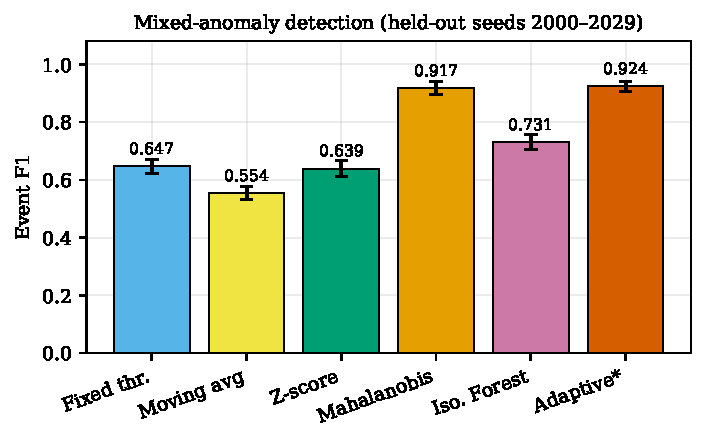
\includegraphics[width=0.72\linewidth]{fig_main_f1.pdf}
  \caption{Event $F_1$ by detector on the held-out mixed scenario. The
  multivariate detectors clear the single-feature baselines by a wide margin.}
  \label{fig:main}
\end{figure}

The per-attack-type breakdown (Figure~\ref{fig:pertype}) explains the gap.
Volumetric events --- floods and bursts --- are caught by almost everything. Port
scans and protocol shifts are caught only by the multivariate detectors and are
completely missed by the volume monitors. Slow ramps are the hardest family for the
proposed detector, because a gradual change is partly absorbed by its own
adaptation; the Isolation~Forest handles ramps best.

\begin{figure}[t]
  \centering
  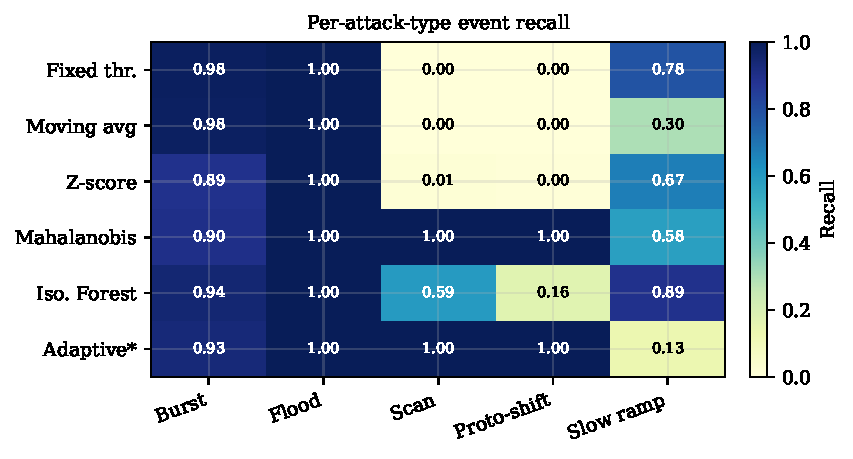
\includegraphics[width=0.72\linewidth]{fig_pertype.pdf}
  \caption{Per-attack-type event recall. The multivariate detectors are the only
  ones that see port scans and protocol shifts; slow ramps are the proposed
  detector's weak point.}
  \label{fig:pertype}
\end{figure}

The decisive result is under non-stationarity (Figure~\ref{fig:drift}). As benign
traffic drifts, the static detectors degrade --- static Mahalanobis falls from
$0.917$ to $0.796$ and the volume monitors fall further --- while the proposed
detector stays essentially flat at about $0.92$.

\begin{figure}[t]
  \centering
  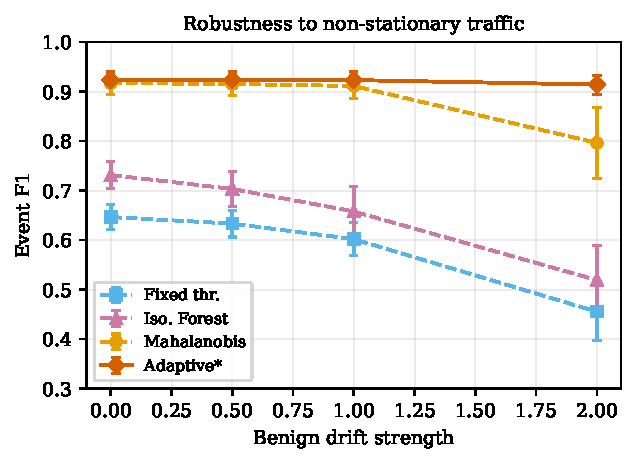
\includegraphics[width=0.58\linewidth]{fig_drift.pdf}
  \caption{Robustness to non-stationary benign traffic. The static detectors
  degrade as drift grows; the proposed online detector holds.}
  \label{fig:drift}
\end{figure}

On real CIC-IDS2017 traffic (Figure~\ref{fig:roc}, Table~\ref{tab:cic}) the
simulated finding reappears: on the non-volumetric port scan the multivariate
detectors are near-perfect (ROC-AUC $0.999$, recall $1.0$) while the volume
monitors miss most of it (recall $0.4$). The DDoS capture is an easy volumetric
case that even the fixed threshold detects perfectly.

\begin{figure}[t]
  \centering
  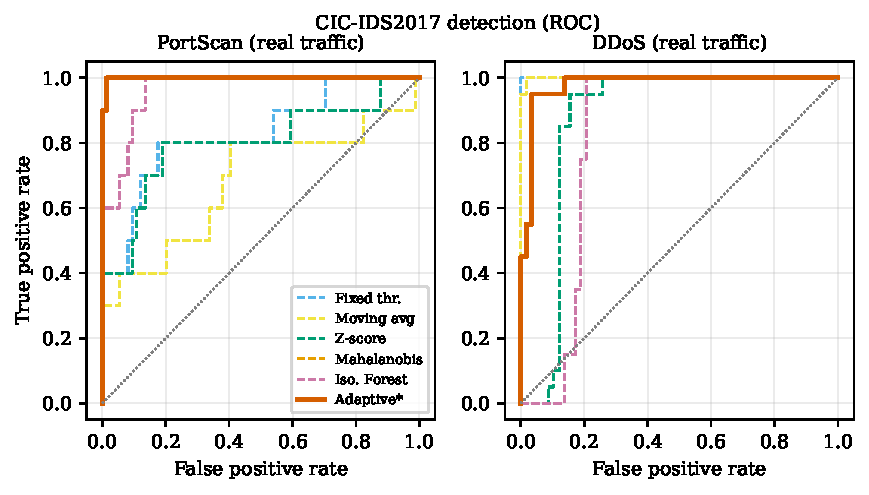
\includegraphics[width=0.9\linewidth]{fig_roc_cic.pdf}
  \caption{ROC curves on real CIC-IDS2017 traffic. The multivariate detectors
  dominate on the port scan; the DDoS is easy for all volume-aware detectors.}
  \label{fig:roc}
\end{figure}

\begin{table}[t]
  \centering
  \caption{CIC-IDS2017 detection (method frozen; threshold calibrated on benign).
  Recall is measured at a $5\%$ benign-calibrated operating point.}
  \label{tab:cic}
  \begin{tabular}{lcccc}
    \toprule
    & \multicolumn{2}{c}{PortScan} & \multicolumn{2}{c}{DDoS} \\
    \cmidrule(lr){2-3}\cmidrule(lr){4-5}
    Detector & ROC-AUC & Recall & ROC-AUC & Recall \\
    \midrule
    Fixed threshold & 0.83 & 0.40 & 1.00 & 1.00 \\
    Moving average & 0.68 & 0.40 & 1.00 & 1.00 \\
    Z-score (static) & 0.80 & 0.40 & 0.87 & 0.00 \\
    Mahalanobis (static) & \textbf{0.999} & \textbf{1.00} & 0.98 & 0.95 \\
    Isolation Forest & 0.96 & 0.60 & 0.82 & 0.00 \\
    \textbf{Adaptive (proposed)} & \textbf{0.999} & \textbf{1.00} & 0.98 & 0.95 \\
    \bottomrule
  \end{tabular}
\end{table}

% =====================================================================
% 7 DISCUSSION
% =====================================================================
\section{Discussion}
The results tell a consistent and deliberately narrow story. The large, reliable
win is from using several features instead of one: both multivariate detectors
see the attacks that volume monitors cannot, on simulated and on real traffic.
This is a property of multi-feature statistical scoring in general, not of the
proposed detector specifically, and we report it as such. The proposed detector's
own contribution is narrower. In stationary traffic it is statistically tied with
the much simpler static Mahalanobis baseline, so online adaptation is unnecessary
when normal traffic does not move. Its value appears only when traffic is
non-stationary, where a frozen model slowly mis-calibrates and drifts into false
alarms while the online model tracks the benign change and holds its operating
point --- which is exactly the regime of a monitor calibrated once and left
running for days. The slow-ramp weakness is the flip side of the same mechanism:
adaptation that helps against benign drift also partly absorbs a slow attack.

% =====================================================================
% 8 COMPARATIVE ANALYSIS
% =====================================================================
\section{Comparative Analysis}
Relative to the four single-feature baselines, the proposed detector is
unambiguously better, by $0.19$ to $0.37$ event $F_1$ with significance at
$p < 10^{-4}$ and a win on all thirty held-out seeds, because those baselines
cannot represent non-volumetric attacks. Relative to the static Mahalanobis
baseline it trades a statistically insignificant difference in stationary
conditions (event $F_1$ $0.924$ versus $0.917$, $p = 0.90$) for a clear,
significant advantage under drift ($+0.118$, $p = 0.002$, winning on
twenty-two of thirty seeds). Relative to the Isolation~Forest --- the only other
multi-feature detector --- it is both more accurate on the mixed scenario
($0.924$ versus $0.731$) and far lighter in state.

Table~\ref{tab:overhead} compares per-window cost and model state. The proposed
detector keeps $72$ floating-point values, about $167$ times less than the
Isolation~Forest's ensemble, and needs no training. Its per-window compute of
about $33\,\mu$s, dominated by an $8\times8$ matrix solve, is the highest of the
six but still far inside a real-time budget for one-second windows --- on the
order of thirty thousand windows per second on a single core. ``Lightweight''
therefore holds on the dimensions that constrain a long-running monitor --- memory
and the absence of retraining --- rather than on raw per-window arithmetic.

\begin{table}[t]
  \centering
  \caption{Per-window compute and model state (lower is lighter).}
  \label{tab:overhead}
  \begin{tabular}{lcc}
    \toprule
    Detector & Time ($\mu$s / window) & State (floats) \\
    \midrule
    Fixed threshold & 0.26 & 1 \\
    Moving average & 0.66 & 60 \\
    Z-score (static) & 0.30 & 2 \\
    Mahalanobis (static) & 3.9 & 72 \\
    Isolation Forest & 9.0 & 12{,}040 \\
    \textbf{Adaptive (proposed)} & 32.8 & 72 \\
    \bottomrule
  \end{tabular}
\end{table}

% =====================================================================
% 9 ABLATION / STATISTICAL ANALYSIS
% =====================================================================
\section{Ablation / Statistical Analysis}
Figure~\ref{fig:ablation} ablates the proposed detector's design on a stationary
and a drifted scenario. Removing the gated update is the most damaging change
(event $F_1$ falls from $0.91$ to $0.82$): without it, attack windows are absorbed
into the model and the detector goes blind. Loosening the covariance gate so that
more windows enter the covariance is almost as harmful, which confirms that
freezing the covariance on suspect windows --- not merely the mean --- is
necessary. Replacing the full covariance with a diagonal one costs most under
drift ($0.916 \to 0.793$) and raises false alarms, showing that the correlations
between features carry real signal. The two optional post-filters do not help:
$m$-of-$n$ persistence is marginally worse, and CUSUM is much worse
($\to 0.30$) because it accumulates on benign flash crowds and fires on them.

\begin{figure}[t]
  \centering
  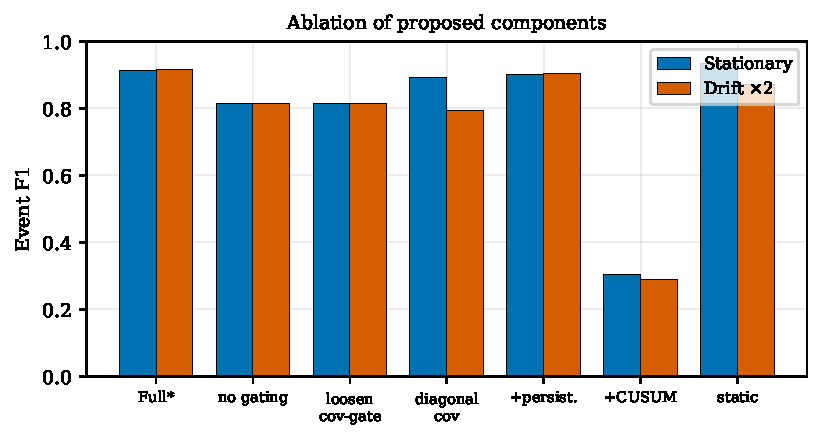
\includegraphics[width=0.82\linewidth]{fig_ablation.pdf}
  \caption{Ablation of the proposed components in stationary and drifted traffic.
  The gated update and the full covariance carry the performance; persistence and
  CUSUM do not help.}
  \label{fig:ablation}
\end{figure}

All comparisons in Sections~6 and~8 are supported by paired Wilcoxon signed-rank
tests over the same thirty held-out seeds, with Holm correction applied across
the five baselines within each setting. The proposed detector's advantage over the
single-feature baselines is significant at $p < 10^{-4}$ in every setting; its
difference from static Mahalanobis is not significant in the stationary case
($p = 0.90$) and is significant at the strongest drift ($p = 0.002$). The
sensitivity sweeps over attack intensity and benign noise (not reproduced here for
space) show the multivariate pair on top throughout, with the proposed detector
marginally behind static Mahalanobis at the highest intensities and marginally
ahead under the heaviest noise.

% =====================================================================
% 10 LIMITATIONS
% =====================================================================
\section{Limitations}
Several limits bound these claims. The controlled experiments use synthetic
traffic, so absolute numbers reflect our generative assumptions rather than any
particular production network; the real-data validation mitigates this but is
itself limited. The CIC-IDS2017 captures are single, hour-long sessions with
minute-resolution timestamps, which forces coarse one-minute windows, yields few
attack windows, and is too short and too stationary to exhibit the drift on which
the proposed detector's advantage rests --- so that advantage is at present shown
only in simulation. The detector also trails on very slow attacks, and its
per-window matrix solve, while real-time here, would need an incremental-inverse
implementation to scale to very high-dimensional feature sets.

% =====================================================================
% 11 CONCLUSION
% =====================================================================
\section{Conclusion}
We asked whether a lightweight, training-free statistical detector can catch the
anomalies that volume monitors miss while staying robust to changing traffic. The
answer is a qualified yes. Multi-feature statistical scoring is what defeats
non-volumetric attacks such as port scans and protocol shifts, on both simulated
and real traffic, and it does so with a few dozen parameters and no training.
Online adaptation on top of that scoring is not needed in stationary conditions,
where it ties the simplest multivariate baseline, but it is what keeps the
detector accurate and calm when normal traffic drifts, which is the realistic
regime for a monitor left running over days.

% =====================================================================
% 12 FUTURE WORK
% =====================================================================
\section{Future Work}
The clearest next step is a real-data drift study on multi-day captures, which
would let the drift advantage be measured outside simulation. The slow-ramp
weakness invites a two-timescale variant that pairs a fast-adapting and a
slow-adapting model so that gradual attacks are not absorbed. Finally, an
incremental update of the covariance inverse would remove the per-window matrix
solve and let the feature set grow without raising cost.

% =====================================================================
% BACK MATTER
% =====================================================================
\section*{Acknowledgment}
The authors thank the Department of Artificial Intelligence \& Data Science,
Chaitanya Bharathi Institute of Technology, and the Computer Networks course
faculty for their guidance on this mini-project.

\section*{Conflict of Interest}
The authors declare that they have no conflict of interest.

\section*{Data Availability}
The CIC-IDS2017 dataset is publicly available from the Canadian Institute for
Cybersecurity. All simulation code, the real-data processing pipeline, result
tables, and figure-generation scripts produced for this project are available in
the accompanying project repository.

\begin{thebibliography}{9}
\small
\bibitem{chandola} V.~Chandola, A.~Banerjee, and V.~Kumar. Anomaly detection: A
survey. \emph{ACM Computing Surveys}, 41(3):1--58, 2009.
\bibitem{ahmed} M.~Ahmed, A.~N.~Mahmood, and J.~Hu. A survey of network anomaly
detection techniques. \emph{Journal of Network and Computer Applications},
60:19--31, 2016.
\bibitem{ring} M.~Ring, S.~Wunderlich, D.~Scheuring, D.~Landes, and A.~Hotho. A
survey of network-based intrusion detection data sets. \emph{Computers \&
Security}, 86:147--167, 2019.
\bibitem{roberts} S.~W.~Roberts. Control chart tests based on geometric moving
averages. \emph{Technometrics}, 1(3):239--250, 1959.
\bibitem{page} E.~S.~Page. Continuous inspection schemes. \emph{Biometrika},
41(1--2):100--115, 1954.
\bibitem{isoforest} F.~T.~Liu, K.~M.~Ting, and Z.-H.~Zhou. Isolation Forest. In
\emph{Proc. 8th IEEE Int. Conf. on Data Mining (ICDM)}, pages 413--422, 2008.
\bibitem{cicids} I.~Sharafaldin, A.~H.~Lashkari, and A.~A.~Ghorbani. Toward
generating a new intrusion detection dataset and intrusion traffic
characterization. In \emph{Proc. 4th Int. Conf. on Information Systems Security
and Privacy (ICISSP)}, pages 108--116, 2018.
\bibitem{engelen} G.~Engelen, V.~Rimmer, and W.~Joosen. Troubling the CIC-IDS-2017
dataset: Errors and lessons learned. In \emph{IEEE Security and Privacy
Workshops}, 2021.
\end{thebibliography}

\end{document}
